\section{Zielsetzung}
\label{sec:Zielsetzung}

In diesem Versuch soll das Emissionsspektrum einer Kupfer-Rötgenröhre und 
fünf Absorptionsspektren verschiedener Elemente mithilfe des Versuchsaufbaus
aufgenommen und untersucht werden.

\section{Theorie}
\label{sec:Theorie}

\subsection{Röntgenstrahlung}

Um Röntgenstrahlen zu erzeugen, wird der glühelektrische Effekt verwendet.\\
Es wird eine Glühkathode stark genug erhitzt, sodass sich eine Wolke aus freien
Elektronen um den Glühdraht der Kathode bildet.\\
Diese werden durch ein elektrisches Feld hin zu einer Anode beschleunigt.
Um Stöße und somit Energieverluste zu vermeiden, befinden sich sowohl Kathode
als auch Anode in einer evakuierten Röhre.\\
Beim Auftreffen auf die Anode entsteht dann schließlich Röntgenstrahlung.\\

\subsubsection{Rötgenspektren}

Röntgenstrahlung besteht aus zwei verschiedenen Spektren. Das 
eine ist das kontinuierliche Bremsspektrum und das andere ist die
vergleichsweise diskrete charakteristische Röntgenstrahlung.\\
Bremsstrahlung entsteht durch das Abbremsen von den beschleunigten
Elektronen am Coloumbfeld eines Atoms des Anodenmaterials. Das Elektron
verliert beim abbremsen an kinetischer Energie, welche in Form von Photonen
emittiert wird.\\
Dadurch, dass die Elektronen je nach Distanz zum Atom unterschiedlich stark
abgebremst werden, ist das Intensitätsspektrum der Bremsstrahlung
kontinuierlich.\\
Die maximale Energie die dabei in Form von Photonen emittiert werden kann, ist die
kinetische Energie des Elektrons. Die minimale Wellenlänge ist somit
\begin{equation}
    \label{eqn:Energiedifferenz}
    \lambda_{\mathrm{min}} = \frac{h\cdot c}{e_0 \cdot U}
\end{equation}
Hier wird also die gesamte kinetische Energie $e_0 \cdot U$ in Strahlungsenergie $h \cdot f$
umgewandelt.\\
\\
Um charakteristische Rötgenstrahlung zu erhalten, wird das Anodenmaterial so ionisiert,
dass eine Leerstelle in einer inneren Schale entsteht. Ein Elektron aus einer äußeren
Schale fällt dann unter Emission einer spezifischen Energie in die innere Schale zurück.\\
Die emittierte charakteristische Energie entspricht in diesem Fall der Energiedifferenz
der beiden Schalen: $h \cdot f = E_{\mathrm{m}} - E_{\mathrm{n}}$. $E_{\mathrm{m}}$ ist hierbei
die Energie der äußeren Schale und $E_{\mathrm{n}}$ die Energie der inneren Schale.\\
Man erwartet hier nun sehr schmale Intensitätsspektren, da die Wellenlänge nur bestimmte
Werte anhand der Gleichung annehmen kann. Im Experiment ist jedoch zu sehen, dass man
bei bestimmten Energien noch kleinere Peaks oben auf dem Hauptpeak erkenne kann.\\
Diese lassen sich dadurch erklären, dass die äußeren Elektronen aufgrund des Bahndrehimpulses
und des Elektronenspins leicht unterschiedliche Bindungsenergien besitzen. Jede charakteristische
Linie ist daher in der Regel in eine Reihe von eng beineinander liegende Linien aufgespalten.
Dieses Erscheinungsbild nennt sich Feinstruktur.\\
Die einzelnen Linien werden mit Buchstaben $K_{\alpha}, K_{\beta}, L_{\alpha}, ...$ benannnt. 
K, L, M, ... stehen hierbei jeweils für die einzelnen Schalen des Atoms, wo die Übergänge
enden und die griechischen Buchstaben definieren woher das äußere Elektron kam.\\
\\
In einem Mehrelektronenatom (, also jedes außer Wasserstoff) schirmen die äußeren
Elektronen und die Wechselwirkung der Elektronen untereinander die Kerladung ab. Dadurch
wird die elektrische Anziehung des Kerns auf die äußeren Elektronen gemindert und die Bindungsenergie
gedämpft. Für diese gilt dann in der n-ten Schale:
\begin{equation}
    \label{eqn:Bindungsenergie}
    E_n = -R_{\infty} z_{\mathrm{eff}}^2 \cdot \frac{1}{n^2}.
\end{equation}
$z_{\mathrm{eff}} = z - \sigma$ bezeichnet hier die effektive Kernladung mit der 
Abschirmkonstante $\sigma$ und der Rydbergenergie $R_{\infty} = 13.6 \si{\electronvolt}$.
Durch die effektive Kerladung wird somit auch der Abschirmeffekt berücksichtig.\\
Bei dem Versuch wird eine Kupferanode verwendet, wo eine $\mathrm{Cu-K}_\alpha$- und eine
$\mathrm{Cu-K}_\beta$-Linie zu erkennen ist, die mit dem kontinuierlichen Spektrum der
Bremsstrahlung überlagert ist.

\subsubsection{Absorption der Rötgenstrahlung}

Bei dem Prozess der Absorption der Rötgenstrahlung bei Energien unter
1 MeV ist der Comptoneffekt und der Photoeffekt die überwiegend dominanten
Prozesse.\\
Der Absorptionskoeffizient nimmt mit steigender Energie immer weiter ab,
nimmt jedoch sprunghaft zu sobald die Photonenenergie gerade größer als die
Bindungsenergie eines Elektrons der inneren Schale ist. Diese Relation ist In
\autoref{Abb:Absorption} zu sehen. Die einzelnen kleineren Kanten, lassen
sich durch die Feinstruktur erklären.\\
\begin{figure}
    \centering
    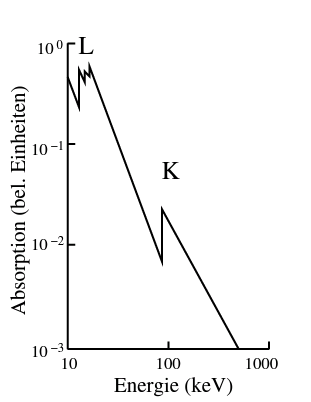
\includegraphics[width=0.3\textwidth]{Bilder/Absorption.png}
    \caption{Maß der Absorption aufgetragen gegen die Energie der Photonen \cite{sample}.}
    \label{Abb:Absorption}
\end{figure}
Die markanten Kanten sind an den Stellen, wo die Gleichung $h f_{\mathrm{abs}} = E_{\mathrm{n}} - E_{\infty}$
erfüllt ist. Diese Kanten werden Absorptionskante genannt.\\
Im Experiment kann die Energie $E$ der Rötgenstrahlung über die Relation $\lambda = cf$ und
durch die Interferenz an einem Kristall untersucht werden.\\
das Röntgenlicht fällt auf einen Kristall, ein dreidimensionales Gitter,
und wird an jedem Atom des Gitters gebeugt. Dadurch interferieren die 
Strahlen miteinander.\\
Bei dem sogenannten Glanzwinkel $\theta$ interferieren die Röntgenstrahlen konstruktiv
miteinander. Mit bekannter Gitterkonstante $d$ ergibt sich dann die Braggsche Bedingung mit
\begin{equation}
    2d \sin{\theta} = n \lambda.
\end{equation}
Durch diese Gleichung kann die Wellenlänge $\lambda$ bestimmt werden. $n$ ist 
die Beugungsordnung.\\
